\chapter{Evaluation}
\label{sec:Evaluation}

\section{Test Environment}
For the purpose of evaluation, the crill cluster at the Research and Computing Center of the University of Houston was used.

\subsection{Crill Cluster Hardware Specification}
\begin{itemize}
\item \textbf{16 NLE Systems nodes (crill-001 - crill-016)}\\
  Four 2.2 GHz 12-core AMD Opteron processors (48 cores total)\\
  64 GB main memory\\
  Two dual-port 4xDDR InfiniBand HCAs

\item \textbf{2 Appro 1326G4 nodes (crill-101 - crill-102)}\\
  Two 2.2 GHz 12-core AMD Opteron processors (24 cores total)\\
  32 GB main memory\\
  Four NVIDIA Tesla M2050 GPUs (448 cores each)\\
  4xDDR InfiniBand HCA

\item \textbf{4 HP DL 160 Gen 8 nodes (crill-200 - crill-203)}\\
  Two 2.4 GHz quad-core Intel Xeon E5-2665 processors (24 cores total)\\
  8 GB main memory\\
  4xDDR InfiniBand HCA
  
\item \textbf{Network Interconnect}\\
  144 port 4xInfiniBand DDR Voltaire Grid Director ISR 2012 switch (shared with whale cluster)\\
  24 port 4xInfiniBand SDR switch (I/O switch to the SSD storage)\\
  48 port Netgear GE switch

\item \textbf{Storage}\\
  2 TB RamSan 620 SSD storage (/pvfs2-ssd)\\
  20 TB Sun StorageTek 6140 array (/home shared with shark cluster)\\
  8 TB distributed PVFS2 storage (/pvfs2)
  
\end{itemize}

\subsection{Crill Cluster Nodes Software Specification}
\begin{itemize}
\item \textbf{Operating System}\\
  Linux kernel version 3.11.10-21-desktop\\
  Distribution: openSUSE 13.1 (x86\_64)
\item \textbf{Open MPI} version 1.8
\item \textbf{HPX} version 0.9.10 release
\item \textbf{Boost} version 1.55.0
\item \textbf{GCC and G++} version 4.8.1
\end{itemize}


\section{Configuration, Compilation, and Execution}

\subsection{Open MPI Configuration Parameteres}
For running different test cases, our evaluation is mostly focused on comparison between Open MPI using ORTE vs. Open MPI using HPX-RTE as runtime.
Listing \ref{lst:config-hpxrte} shows the configure line for the Open MPI installation. The only parameter that needs to be changed is \verb|--with-orte|. When this parameter is set to ``yes'', Open MPI uses ORTE as runtime. If we set this parameter to ``no'', Open MPI will use HPX-RTE.

\begin{lstlisting}[language=C, frame=single, basicstyle=\footnotesize, caption=Configure Line of Open MPI with HPX-RTE\label{lst:config-hpxrte}]
  $ ./configure CFLAGS=``-g -O0'' CXXFLAGS=``-g -O0''
    --prefix=/home/hadi/opt/openmpi
    --with-hpx=/opt/hpx-0.9.10-release
    --with-boost=/opt/boost/1-55-0
    --disable-vt --enable-mca-no-build=coll-ml,vprotocol
    --enable-oshmem=no --enable-mpi-profile=no
    --enable-static --with-orte=no
\end{lstlisting}

\subsection{Compiling MPI Applications}
Listing \ref{lst:compile} illustrates the compile line for our Hello World example. This line could be integrated into Open MPI software in future iterations of the development. Therefore, users will not have to manually insert all the compile and linkage flags needed. The same command can be used when ORTE is the installed runtime.

\begin{lstlisting}[language=C, frame=single, basicstyle=\footnotesize, caption=Compile Line for Hello World\label{lst:compile}]
  $ mpicxx -o mpi_hello mpi_hello.c -rdynamic -fPIC -std=c++11
  -Wall -Wno-unused-local-typedefs -Wno-strict-aliasing
  -Wsign-promo -Wno-cast-align -Werror=vla -Werror=return-type
  -fdiagnostics-show-option  -Werror=uninitialized -pthread
  -DHPX_DEBUG -D_GNU_SOURCE  -I${HPX_DIR}/include/hpx/external
  -I${HPX_DIR}/include -I/usr/include/google
  -DHPX_APPLICATION_EXPORTS -DHPX_ENABLE_ASSERT_HANDLER
  -DHPX_DEBUG -finline-functions -I/opt/boost/1-55-0/include
  -L/opt/boost/1-55-0/lib -Wl,-rpath,:${HPX_DIR}/lib/hpx
  -L${HPX_DIR}/lib/hpx -L${HPX_DIR}/lib -lhpx -lhpx_init
  -lhpx_serialization -lboost_date_time -lboost_filesystem
  -lboost_program_options -lboost_regex -lboost_serialization
  -lboost_system -lboost_thread -lboost_atomic -lboost_chrono
  -lprofiler -liostreams -L/lib64 -lrt -ldl -lutil -g -O0
\end{lstlisting}

\subsection{Running MPI Applications}

For running applications using ORTE, we will use ``mpirun'' command, which is a soft link to ``orterun'' command. This is shown in listing \ref{lst:orterun}.

\begin{lstlisting}[language=C, frame=single, basicstyle=\footnotesize, caption=Running MPI Applications Using ORTE \label{lst:orterun}]
$ mpirun -np 1 -pernode ./mpi_hello
\end{lstlisting}

HPX provides support for Slurm (Simple linux utility for resource management)~\cite{yoo2003slurm}. To run applications using HPX-RTE, we use ``srun'' command. Listing \ref{lst:hpxrte-run} demonstrates an example.

\begin{lstlisting}[language=C, frame=single, basicstyle=\footnotesize, caption=Running MPI Applications Using HPX-RTE \label{lst:hpxrte-run}]
$ srun -N 1  -n 1 --ntasks-per-node=1 ./mpi_hello --hpx:run-hpx-main
  --hpx:threads=2
\end{lstlisting}

\iffalse

\section{Evaluation}

In our evaluations, there are two ways to measure the time in the case of each application: The total time measured by the ``time'' command in Linux (Listing \ref{lst:hpxrte-run} nad \ref{lst:orterun}), and measuring the time within the application. The time reported by the application is reported on a per process basis. Numbers reported in this section are averge numbers reported by the application when the application reported times are reported.

Every test was run at lesat three times. The average of all three times is reported.

\subsection{MPI Hello World}

\begin{figure}[h!]
\centering
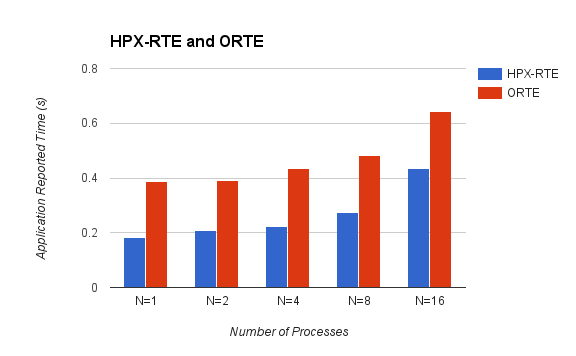
\includegraphics[scale=0.7]{images/time-app-hello-world-infiniband.png}
\caption[Application Reported Time - Hello World - Infiniband]{Application Reported Time - Hello World - Infiniband}
\label{fig:time-app-hello-world-infiniband}
\end{figure}

%srun -N 2 -n 2 -c 2 ./mpi_hello --hpx:run-hpx-main --hpx:threads=2

\subsection{Heat Solver}
~\cite{resch1999comparison}

\begin{figure}[h!]
\centering
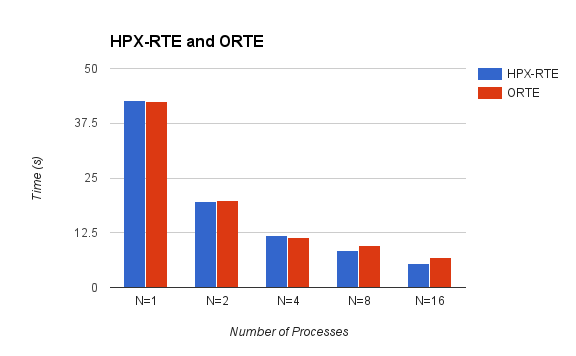
\includegraphics[scale=0.7]{images/time-all-heatsolver-80-infiniband.png}
\caption[Application Reported Time - Hello World - Infiniband]{Time - Heat Solver - Problem Size 80x80x80 - Infiniband}
\label{fig:time-all-heatsolver-80-infiniband.png}
\end{figure}

\begin{figure}[h!]
\centering
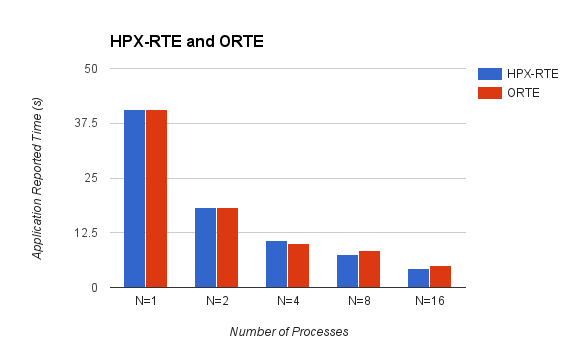
\includegraphics[scale=0.7]{images/time-app-heatsolver-80-infiniband.png}
\caption[Application Reported Time - Hello World - Infiniband]{Application Reported Time - Heat Solver - Problem Size 80x80x80 - Infiniband}
\label{fig:time-app-heatsolver-80-infiniband.png}
\end{figure}


\subsection{Code Size}

NAS parallel benchmarks~\cite{bailey1991parallel}

\fi
